% Options for packages loaded elsewhere
\PassOptionsToPackage{unicode}{hyperref}
\PassOptionsToPackage{hyphens}{url}
%
\documentclass[
]{book}

\usepackage{amsmath,amssymb}
\usepackage{iftex}
\ifPDFTeX
  \usepackage[T1]{fontenc}
  \usepackage[utf8]{inputenc}
  \usepackage{textcomp} % provide euro and other symbols
\else % if luatex or xetex
  \usepackage{unicode-math}
  \defaultfontfeatures{Scale=MatchLowercase}
  \defaultfontfeatures[\rmfamily]{Ligatures=TeX,Scale=1}
\fi
\usepackage{lmodern}
\ifPDFTeX\else  
    % xetex/luatex font selection
\fi
% Use upquote if available, for straight quotes in verbatim environments
\IfFileExists{upquote.sty}{\usepackage{upquote}}{}
\IfFileExists{microtype.sty}{% use microtype if available
  \usepackage[]{microtype}
  \UseMicrotypeSet[protrusion]{basicmath} % disable protrusion for tt fonts
}{}
\makeatletter
\@ifundefined{KOMAClassName}{% if non-KOMA class
  \IfFileExists{parskip.sty}{%
    \usepackage{parskip}
  }{% else
    \setlength{\parindent}{0pt}
    \setlength{\parskip}{6pt plus 2pt minus 1pt}}
}{% if KOMA class
  \KOMAoptions{parskip=half}}
\makeatother
\usepackage{xcolor}
\setlength{\emergencystretch}{3em} % prevent overfull lines
\setcounter{secnumdepth}{2}
% Make \paragraph and \subparagraph free-standing
\makeatletter
\ifx\paragraph\undefined\else
  \let\oldparagraph\paragraph
  \renewcommand{\paragraph}{
    \@ifstar
      \xxxParagraphStar
      \xxxParagraphNoStar
  }
  \newcommand{\xxxParagraphStar}[1]{\oldparagraph*{#1}\mbox{}}
  \newcommand{\xxxParagraphNoStar}[1]{\oldparagraph{#1}\mbox{}}
\fi
\ifx\subparagraph\undefined\else
  \let\oldsubparagraph\subparagraph
  \renewcommand{\subparagraph}{
    \@ifstar
      \xxxSubParagraphStar
      \xxxSubParagraphNoStar
  }
  \newcommand{\xxxSubParagraphStar}[1]{\oldsubparagraph*{#1}\mbox{}}
  \newcommand{\xxxSubParagraphNoStar}[1]{\oldsubparagraph{#1}\mbox{}}
\fi
\makeatother


\providecommand{\tightlist}{%
  \setlength{\itemsep}{0pt}\setlength{\parskip}{0pt}}\usepackage{longtable,booktabs,array}
\usepackage{calc} % for calculating minipage widths
% Correct order of tables after \paragraph or \subparagraph
\usepackage{etoolbox}
\makeatletter
\patchcmd\longtable{\par}{\if@noskipsec\mbox{}\fi\par}{}{}
\makeatother
% Allow footnotes in longtable head/foot
\IfFileExists{footnotehyper.sty}{\usepackage{footnotehyper}}{\usepackage{footnote}}
\makesavenoteenv{longtable}
\usepackage{graphicx}
\makeatletter
\def\maxwidth{\ifdim\Gin@nat@width>\linewidth\linewidth\else\Gin@nat@width\fi}
\def\maxheight{\ifdim\Gin@nat@height>\textheight\textheight\else\Gin@nat@height\fi}
\makeatother
% Scale images if necessary, so that they will not overflow the page
% margins by default, and it is still possible to overwrite the defaults
% using explicit options in \includegraphics[width, height, ...]{}
\setkeys{Gin}{width=\maxwidth,height=\maxheight,keepaspectratio}
% Set default figure placement to htbp
\makeatletter
\def\fps@figure{htbp}
\makeatother

%%% load packages
\usepackage{geometry}
\usepackage{xcolor}
\usepackage{eso-pic}
\usepackage{fancyhdr}
\usepackage[explicit]{titlesec}
\usepackage{marginnote}
\usepackage{setspace}
\usepackage{enumitem}
\usepackage[most]{tcolorbox}




%%% --- Define Colors ---
% Define Colors
\definecolor{my_orange}{HTML}{FF8E00}
\definecolor{blender_blue}{HTML}{236192}
\definecolor{remember_gold}{HTML}{FFDE7E}




%%% --- Adjust Document Settings ---
% Set page size
\geometry{a4paper, left=30mm, top=25mm, bottom=25mm, right=30mm}

% Activate fancy-Style
\pagestyle{fancy}

% Delete default-Styles
\fancyhf{}






%%% --- Adjust Font ---
\renewcommand{\normalsize}{\fontsize{12pt}{14pt}\selectfont}
\makeatletter
\renewcommand\normalsize{%
  \@setfontsize\normalsize{12pt}{15pt}% 12pt Schrift und 15pt Zeilenabstand
  \abovedisplayskip 11pt plus 3pt minus 7pt%
  \abovedisplayshortskip \z@ plus 3pt%
  \belowdisplayshortskip 8pt plus 3pt minus 4pt%
  \belowdisplayskip \abovedisplayskip
  \let\@listi\@listI%
}
\makeatother
\normalsize

% Increase space between lines
\setstretch{1.5}

% Remove spacing after lists
\setlist{nosep}

% Remove spacing for new paragraphs
\setlength{\parskip}{0pt}

% Adjust spacing after titles (\Section, left, before, after)
\titlespacing*{\chapter}{0pt}{0pt}{0pt}
\titlespacing*{\section}{0pt}{10pt}{0pt}
\titlespacing*{\subsection}{0pt}{10pt}{0pt}
\titlespacing*{\subsubsection}{0pt}{10pt}{0pt}





%%% --- Adjust Margins ---
% Change marginnotes
\let\oldmarginnote\marginnote

% Define width off the marings
\setlength{\marginparwidth}{2cm}


\renewcommand{\marginnote}[1]{%
  \oldmarginnote{{\footnotesize\selectfont #1}}%
}





%%% --- Adjust chapter titles ---
% Remove "Chapter"-prefix from chapter-title
%Adjust title format
\titleformat{\chapter}[display]
  % Font of the title
  {\normalfont\huge\bfseries}
  % Suppress Chapter-Number
  {}
  % Remove space after (removed) chapter number
  {0pt}
  % Execute Chapter-title
  {#1}





%%% --- Adjust Page Header ---
% Remove default-Header
\renewcommand{\headrulewidth}{0pt}

% Increase space between header and text
\setlength{\headsep}{30pt}

% Set text for heading
\makeatletter
\renewcommand{\chaptermark}[1]{\markboth{#1}{}}
% Remove "Chapter"-Prefix
\renewcommand{\@chapapp}{}
\makeatother


%%% Odd pages (Recto)
\newcommand{\headerRecto}{%
  % Create orange box
  \colorbox{my_orange}{%
    \makebox[\textwidth][l]{%
      \parbox[t]{\textwidth}{%
        \vspace{5pt}%
        % Create box with page number (20% of page width)
        \makebox[0.20\textwidth][l]{\color{white}\bfseries\thepage}%
        % Create box with chapter (75% of page width)
        \makebox[0.75\textwidth][r]{\color{white}\bfseries\leftmark}%
        \vspace{5pt}%
      }%
    }%
  }%
}

%%% Even pages (Verso)
\newcommand{\headerVerso}{%
  \colorbox{my_orange}{%
    \makebox[\textwidth][l]{%
      \parbox[t]{\textwidth}{%
        \vspace{5pt}%
        % Create box with chapter (75% of page width)
        \makebox[0.75\textwidth][l]{\color{white}\bfseries\leftmark}%
        % Create box with page number (20% of page width)
        \makebox[0.20\textwidth][r]{\color{white}\bfseries\thepage}%
        \vspace{5pt}%
      }%
    }%
  }%
}


%% Asign header to odd pages
\fancyhead[LO,RO]{\headerRecto}

%% Asign header to even pages
\fancyhead[LE,RE]{\headerVerso}

%% Asign header to even pages

%% Overwrite plain-Style at beginning of chapter
\fancypagestyle{plain}{%
  % Remove headers
  \fancyhf{}
  % No additional lines
  \renewcommand{\headrulewidth}{0pt}
  %% Asign header to even pages
  \fancyhead[LO,RO]{\headerRecto}
  %% Asign header to odd pages
  \fancyhead[LE,RE]{\headerVerso}
}





%%% --- Define Boxes ---
%## Tipp-box
% Define new colorbox
\newtcolorbox{tipp}[1]{
% Add space before box and cener box
before=\bigskip\centering,
% Add space after the box
after=\bigskip,
% Activate enhanced mode of colorbox
enhanced,
% Create round corners
arc=10pt,
% Create gold frame
colframe=green!75!black,
% Craete gold background color
colback=green!5!white,
% Define Font of title (black font, sans-serife and large
fonttitle=\sffamily\bfseries\Large,
% Set content 1 as title
title=#1,
% Add space before and after the title inside the box
title={\vspace{2.5mm}#1\vspace{2.5mm}},
% Set space in upper left corner 
leftupper=2.5cm,
% Set round corners
rounded corners,
% Fix title to top of box
attach boxed title to top,
frame hidden,
% Define style of title
boxed title style={
    % Activate enhanced settings of title-field
    enhanced,
    % Set frame of title box
    colframe=green!75!black,
    % Set background of title box
    colback=green!75!black,
    % Set round-angle of title field
    arc=10pt,
    % Supress frame around title fileld
    bottomrule=0pt,
    rightrule=0pt,},
  % Overlay image
  overlay={
    % Set anchor north-west
    \node[anchor=north west] 
      % Adjust position in relation to frame
      at ([xshift=10pt,yshift=-1.75\baselineskip]frame.north west)
        % Add image
       {
\includegraphics[width=1cm]{"icons/info.png"}};}}



%%%%% Exercise
% Define new colorbox
\newtcolorbox[auto counter]{exercise}[2][]{
% Add space before box and cener box
before=\bigskip\centering,
% Add space after the box
after=\bigskip,
% Activate enhanced mode of colorbox
enhanced,
% Create round corners
arc=15pt,
% Create blue frame
colframe=blender_blue,
% Craete blue background color
colback=blender_blue!5!white,
% Define Font of title (black font, sans-serife and large
fonttitle=\sffamily\bfseries\Large,
% Set title
title=Übung~\thetcbcounter,
% Define sharp corners
sharp corners,
% Set space in upper left corner 
leftupper=2.5cm,
% Overlay image
overlay={
  % Set anchor north-west
  \node[anchor=north west] 
    % Adjust position
    at ([xshift=10pt,yshift=-.65\baselineskip]frame.north west)
     % Add image
     {\includegraphics[width=1cm,height=1cm]{"icons/exercise.png"}};},
% Set round corners
rounded corners=northeast,
% Fix title to top of box
attach boxed title to top left,
% Define style of title
boxed title style={
    % Activate enhanced settings of title-field
    enhanced,
    % Set frame of title box
    colframe=blender_blue,
    % Set background of title box
    colback=blender_blue,
    % Set round-angle of title field
    arc=5pt,
    % Supress frame around title fileld
    bottomrule=0pt,
    rightrule=0pt,
    % Set sharp corners
    sharp corners,
    % Set round corners norh-east
    rounded corners=northeast,},
% Define stly of (emtpy) interior block
interior style={},
% Define style of frame
frame style={
    % Set colors
    color= cyan!5!white,
    fill=none},
% Align additional overlays
overlay unbroken and first={
    % Place text
    \node[anchor=west,font=\sffamily\bfseries,color=blue] 
    % Position text east of title and with large font
    at (title.east) {{\Large #2}};
    %
    \node[anchor=north west] 
    % Set position
    at ([xshift=10pt, yshift=-1.75\baselineskip]frame.north west)
      % Add image
     {\includegraphics[width=1.5cm]{"icons/exercise.png"}};},#1}



%%%%% Remember
% Define new colorbox
\newtcolorbox{remember}[1]{
% Add space before box and cener box
before=\bigskip\centering,
% Add space after the box
after=\bigskip,
% Activate enhanced mode of colorbox
enhanced,
% Create round corners
arc=10pt,
% Create gold frame
colframe=remember_gold,
% Craete gold background color
colback=remember_gold,
% Define Font of title (black font, sans-serife and large
fonttitle=\color{black}\sffamily\bfseries\Large,
% Set content 1 as title
title=#1,
% Add space before and after the title inside the box
title={\vspace{2.5mm}#1\vspace{2.5mm}},
% Set space in upper left corner 
leftupper=2.5cm,
% Set round corners
rounded corners,
% Fix title to top of box
attach boxed title to top,
% Define style of title
boxed title style={
    % Activate enhanced settings of title-field
    enhanced,
    % Set frame of title box
    colframe=remember_gold,
    % Set background of title box
    colback=remember_gold,
    % Set round-angle of title field
    arc=10pt,
    % Supress frame around title fileld
    bottomrule=0pt,
    rightrule=0pt
    },
  % Overlay image
  overlay={
    % Set anchor north-west
    \node[anchor=north west] 
      % Adjust position in relation to frame
      at ([xshift=10pt,yshift=-1.75\baselineskip]frame.north west)
        % Add image
       {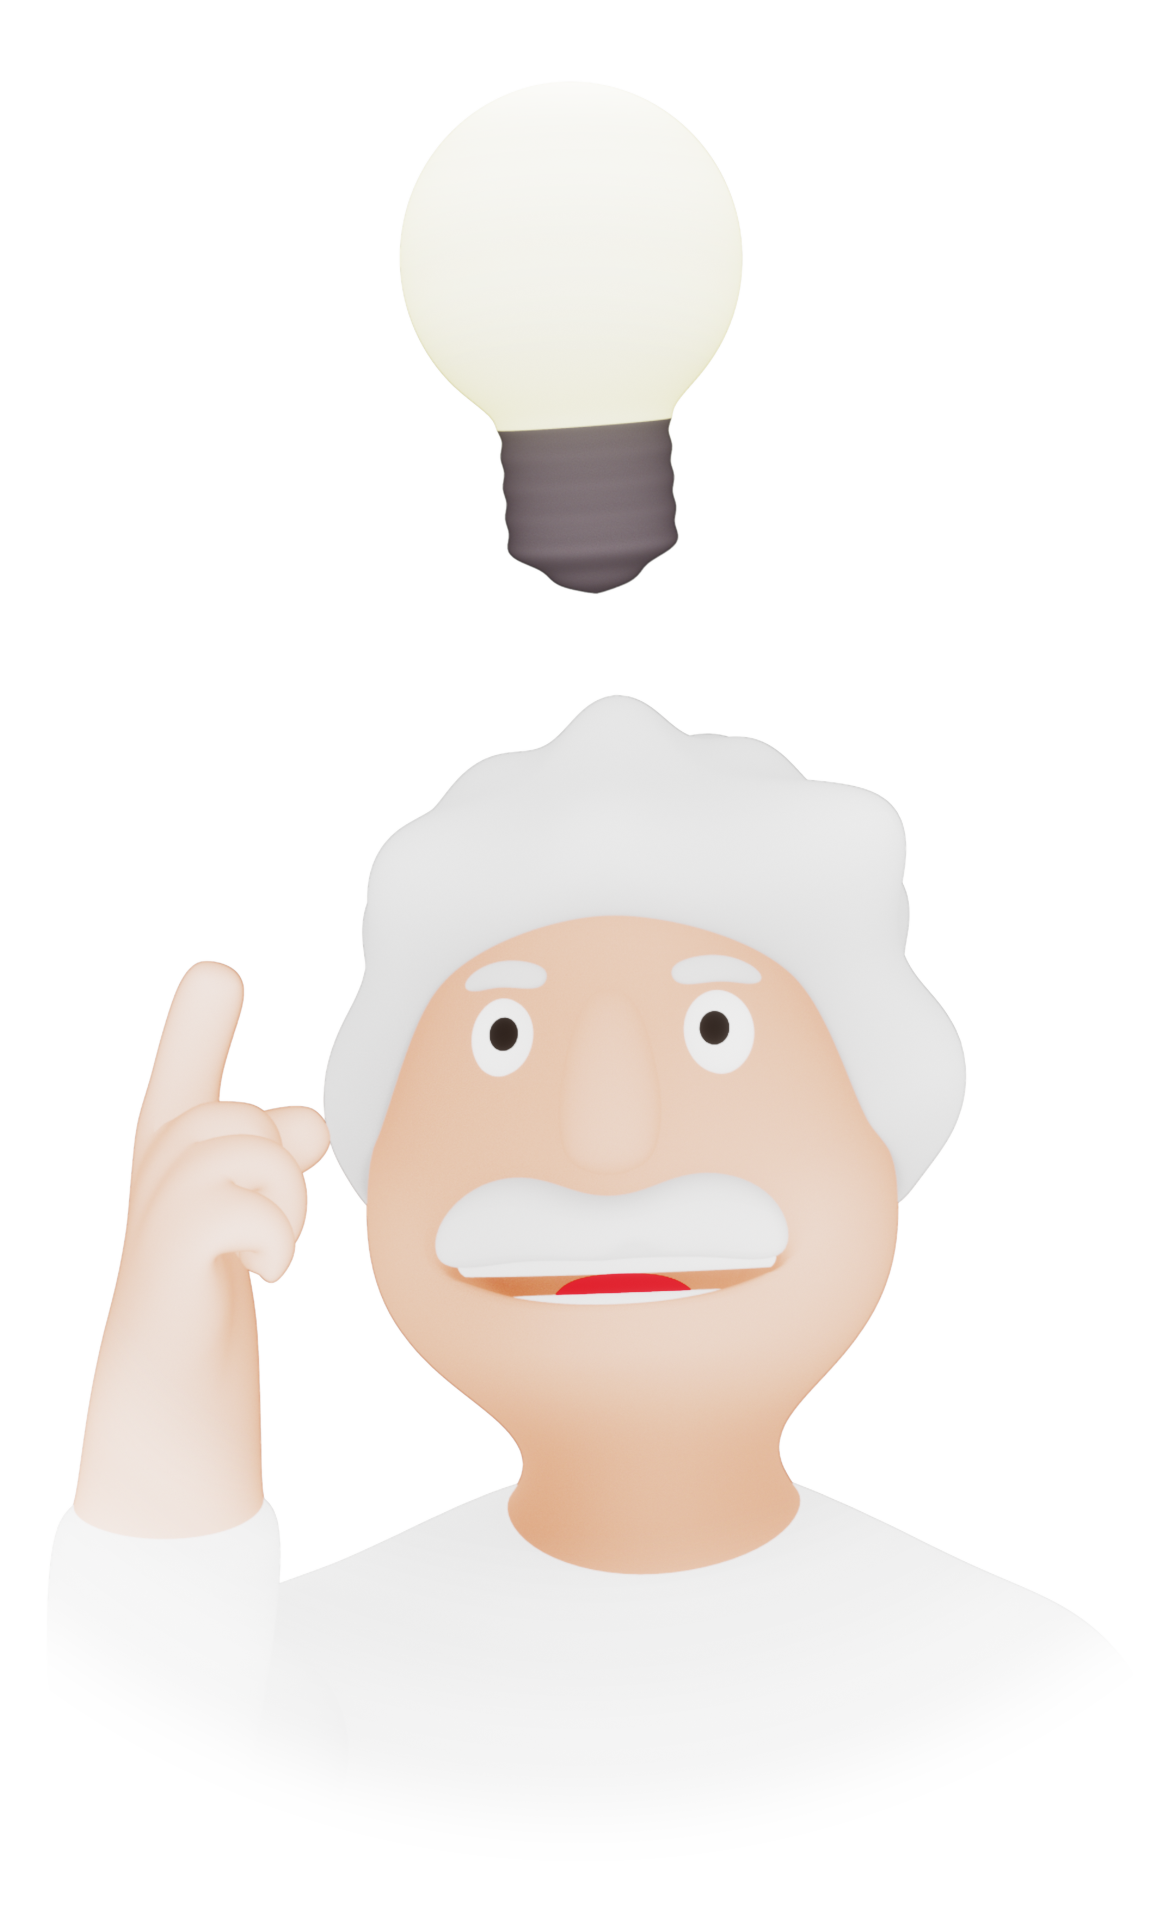
\includegraphics[width=1cm]{"icons/remember.png"}};}}
\renewcommand{\familydefault}{\sfdefault}
\newcommand{\kbd}[1]{\fbox{\texttt{#1}}}
\makeatletter
\@ifpackageloaded{caption}{}{\usepackage{caption}}
\AtBeginDocument{%
\ifdefined\contentsname
  \renewcommand*\contentsname{Inhaltsverzeichnis}
\else
  \newcommand\contentsname{Inhaltsverzeichnis}
\fi
\ifdefined\listfigurename
  \renewcommand*\listfigurename{Abbildungsverzeichnis}
\else
  \newcommand\listfigurename{Abbildungsverzeichnis}
\fi
\ifdefined\listtablename
  \renewcommand*\listtablename{Tabellenverzeichnis}
\else
  \newcommand\listtablename{Tabellenverzeichnis}
\fi
\ifdefined\figurename
  \renewcommand*\figurename{Abbildung}
\else
  \newcommand\figurename{Abbildung}
\fi
\ifdefined\tablename
  \renewcommand*\tablename{Tabelle}
\else
  \newcommand\tablename{Tabelle}
\fi
}
\@ifpackageloaded{float}{}{\usepackage{float}}
\floatstyle{ruled}
\@ifundefined{c@chapter}{\newfloat{codelisting}{h}{lop}}{\newfloat{codelisting}{h}{lop}[chapter]}
\floatname{codelisting}{Listing}
\newcommand*\listoflistings{\listof{codelisting}{Listingverzeichnis}}
\makeatother
\makeatletter
\makeatother
\makeatletter
\@ifpackageloaded{caption}{}{\usepackage{caption}}
\@ifpackageloaded{subcaption}{}{\usepackage{subcaption}}
\makeatother

\ifLuaTeX
\usepackage[bidi=basic]{babel}
\else
\usepackage[bidi=default]{babel}
\fi
\babelprovide[main,import]{ngerman}
% get rid of language-specific shorthands (see #6817):
\let\LanguageShortHands\languageshorthands
\def\languageshorthands#1{}
\ifLuaTeX
  \usepackage{selnolig}  % disable illegal ligatures
\fi
\usepackage{bookmark}

\IfFileExists{xurl.sty}{\usepackage{xurl}}{} % add URL line breaks if available
\urlstyle{same} % disable monospaced font for URLs
\hypersetup{
  pdftitle={Creating the World: Grafik, Design \& Animation},
  pdflang={de},
  hidelinks,
  pdfcreator={LaTeX via pandoc}}


\title{Creating the World: Grafik, Design \& Animation}
\usepackage{etoolbox}
\makeatletter
\providecommand{\subtitle}[1]{% add subtitle to \maketitle
  \apptocmd{\@title}{\par {\large #1 \par}}{}{}
}
\makeatother
\subtitle{(inkl. Einführung in die 3D Modelierung mit Blender)}
\author{}
\date{}

\begin{document}
\frontmatter
\maketitle

\renewcommand*\contentsname{Inhaltsverzeichnis}
{
\setcounter{tocdepth}{1}
\tableofcontents
}

\mainmatter
\begin{tipp}{Blender unterstÃŒtzt nur noch die 64-Bit-Architektur}
Seit der Version 2.81 von Blender werden nur noch Computer mit einer 64-Bit-Architektur unterstÃŒtzt. Microsoft unterstÃŒtzt diese Systeme seit 2020 nicht mehr und auch an-dere Software-Entwickler haben den Support dieser Systeme eingestellt. 
\end{tipp}

\begin{exercise}{Blender unterstÃŒtzt nur noch die 64-Bit-Architektur}
Seit der Version 2.81 von Blender werden nur noch Computer mit einer 64-Bit-Architektur unterstÃŒtzt. Microsoft unterstÃŒtzt diese Systeme seit 2020 nicht mehr und auch an-dere Software-Entwickler haben den Support dieser Systeme eingestellt. 
\end{exercise}

\begin{remember}{Merke...}
Seit der Version 2.81 von Blender werden nur noch Computer mit einer 64-Bit-Architektur unterstÃŒtzt. Microsoft unterstÃŒtzt diese Systeme seit 2020 nicht mehr und auch an-dere Software-Entwickler haben den Support dieser Systeme eingestellt. 
\end{remember}

\chapter{1. Vorbereitung von Blender}\label{vorbereitung-von-blender}

\section{Installation von Blender}\label{installation-von-blender}

\marginnote{Installationsdatei herunterladen}

Um Blender auf einem Rechner zu installieren, muss das
Installationspaket von Blender auf dessen Website
\url{https://www.blender.org/} unter dem Reiter «Download»
heruntergeladen werden. Dort sollte bereits automatisch das
Betriebssystem des Rechners erkannt und die aktuellste Version angeboten
werden. Ansonsten lässt sich mittels eines Auswahlfeldes auch die
entsprechende Version auswählen.

\marginnote{Frühere Versionen von Blender}

Unter \url{https://www.blender.org/download/releases/} lassen sich zudem
frühere Versionen von Blender herunterladen. Dieser Kurs ist auf Blender
3.3 ausgerichtet, weshalb der Download dieser Version empfohlen wird.

\subsection{Mac}\label{mac}

\marginnote{Installationsdatei für Mac-User}

Mac-Benutzer wählen den Link mit der Endung «\emph{.dmg}». Abhängig vom
Computermodell gibt es zwei Versionen. Für Apple-Computer, welche Apples
hauseigenen Prozessor M1 eingebaut haben, wird die Version mit der
Endung «arm64.dmg» benötigt. Für die anderen Apple-Computer die Version
mit der Endung «\emph{x64.dmg}». Um herauszufinden, welcher
Prozessor/Chip im eigenen Apple-Gerät eingebaut ist, kann man im Menü
«\emph{Über diesen Mac}» (oben links beim Apfelsymbol zu finden)
nachschauen. Wenn Apples eigener Chip verbaut ist, wird «\emph{Chip
Apple M1}» aufgelistet. Wenn der Computer nicht über den M1-Chipf
verfügt, wird an dieser Stelle der Prozessor aufgeführt.

\marginnote{Installation}

Nach dem Download sollte das entsprechende .dmg-Paket geöffnet werden.
Anschliessend öffnet sich ein Fenster, dass die Blender-Software und den
Applikationsordner zeigt. Hier sollte nun die Blender-Software in den
Applikationsordner gezogen werden. Anschliessend ist die Installation
abgeschlossen.

\subsection{Windows}\label{windows}

\marginnote{Installation für Windows-User}

Windows-Benutzer können den Link mit der Endung «\emph{.msi}» auswählen.
Nach dem Download kann die Datei geöffnet werden und die Installation
konfiguriert werden.

\marginnote{Blender ohne Installation nutzen}

Es ist auch möglich, Blender ohne eine Installation zu verwenden --
hierfür muss der Link mit der Endung «\emph{.zip}» ausgewählt werden.
Nach dem Extrahieren der Dateien kann Blender über diesen Ordner
gestartet werden. Dadurch kann Blender auf ein externes Speichermedium
transferiert werden und an anderen Computern gestartet werden. Dies hat
allerdings einige Nachteile. Der Computer weiss dadurch etwa nicht, mit
welchem Programm er standardmässig die Dateien von Blender öffnen kann,
und Blender wird auch nicht unter den installierten Programmen
aufgelistet.

\begin{tipp}{Weiterführende Informationen}
Seit der Version 2.81 von Blender werden nur noch Computer mit einer 64-Bit-Architektur unterstützt. Microsoft unterstützt diese Systeme seit 2020 nicht mehr und auch andere Software-Entwickler haben den Support dieser Systeme eingestellt.
\end{tipp}

\section{Der erste Start von Blender}\label{der-erste-start-von-blender}

Beim ersten Start von Blender erscheint ein Quick-Setup-Menü, bei dem
einige Grundeinstellungen eingestellt werden können. Diese können in der
Regel so belassen werden, wie sie sind. Die folgenden Einstellungen
stehen zur Verfügung:

\begin{itemize}
\tightlist
\item
  \textbf{Language}: Hier kann die Sprache eingestellt werden.
\item
  \textbf{Shortcuts}: Hier können die Shortcut-Einstellungen ausgewählt
  werden. Dieser Kurs orientiert sich an der Default-Einstellung
  «\emph{Blender}».
\item
  \textbf{Select with}: Hier kann eingestellt werden, ob jeweils mit der
  linken oder der rechten Maustaste Objekte ausgewählt werden können.
  Dieser Kurs geht davon aus, dass eine Auswahl mit der linken Maustaste
  erfolgt.
\item
  \textbf{Spacebar}: Die Funktion der Leertaste kann drei verschiedenen
  Funktionen zugewiesen werden. Per Default wird die Leertaste
  verwendet, um Animationen zu starten (Option «\emph{Play}»).
  Allerdings kann sie auch der Option «\emph{Tools}» zugewiesen werden.
  Mittels der Einstellung «\emph{Search}» wird durch die Leertaste ein
  Suchfeld geöffnet, mit dem Befehle gesucht werden können. Für diesen
  Kurs spielt es keine grosse Rolle, welche Funktion der Leertaste
  zugewiesen wird. Die Befehlssuche ist allerdings sehr nützlich, kann
  aber alternativ auch mit der Taste \kbd{F3} geöffnet werden.
\item
  \textbf{Theme}: Hier kann das farbliche Layout von Blender angepasst
  werden. Grafiken in diesem Kurs wurden mit dem Theme «\emph{Blender
  Dark}» erstellt.
\end{itemize}

\section{Die Arbeitsoberfläche von
Blender}\label{die-arbeitsoberfluxe4che-von-blender}

\subsection{Das Willkommensfenster}\label{das-willkommensfenster}

\marginnote{Optionen im Willkommensfenster}

Blender begrüsst seine Nutzer mit einem Willkommensfenster. In diesem
Fenster werden die letzten geöffneten Projekte auf der rechten Seite
unter den «\emph{Recent Files}» aufgelistet. Auf der linken Seite des
Willkommensfenster kann unter «\emph{New File}» ein neues Projekt
erstellt werden. Dabei lässt sich die Art des Projekts bereits genauer
definieren. Je nach ausgewählter Projektart werden unterschiedliche
Ansichtsvorlagen geladen.

\begin{figure}

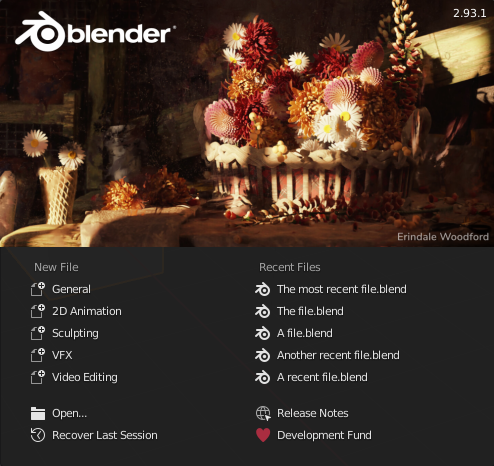
\includegraphics{Chapters/Images/Chapter_1/1_1_Welcome_Screen.png}

\caption{\label{fig-1_1}Willkommensfenster}

\end{figure}%

\marginnote{Auswahl von Ansichtsvorlagen}

Zu den möglichen Ansichtsvorlagen gehören:

\begin{itemize}
\tightlist
\item
  \textbf{General}: Öffnet eine Standardvorlage für das Bearbeiten von
  3D-Objekten.
\item
  \textbf{2D Animation}: Öffnet eine Vorlage zum Erstellen von
  2D-Animationen.
\item
  \textbf{Sculpting}: Öffnet eine Vorlage, welche für das Sculpting von
  Objekten geeignet ist. Dabei werden Objekte anhand von Pinseln direkt
  in ihrer Form verändert.
\item
  \textbf{VFX}: Öffnet eine Vorlage für die Erstellung visueller Effekte
  (VFX), beispielsweise in Videos.
\item
  \textbf{Video Editing}: Öffnet eine Vorlage zum Bearbeiten von Videos.
\end{itemize}

\marginnote{Fokus auf «General»}

Dieser Kurs wird sich auf die 3D-Modellierung fokussieren. Deshalb wird
jeweils die Ansichtsvorlage «\emph{General}» verwendet. Diese Vorlage
ist so generell, dass sie im Hintergrund schon geladen ist, während das
Willkommensfenster dargestellt wird. Deshalb ist es auch möglich,
einfach ausserhalb des Willkommensfensters zu klicken. Dadurch
verschwindet das Willkommensfenster und die General-Vorlage, die bereits
im Hintergrund besteht, wird sichtbar.

\subsection{Die verschiedenen Areale beim
General-Projekt}\label{die-verschiedenen-areale-beim-general-projekt}

\marginnote{Default Editoren}

Die verschiedenen Werkzeuge, welche Blender anbietet, sind innerhalb
verschiedener Editoren aufzufinden. Diese Editoren werden als separate
und austauschbare Areale in Blender dargestellt. Beim Start eines neuen
Projekts (mit der Vorlage General) ist die Ansicht in vier Areale
unterteilt:

\begin{itemize}
\tightlist
\item
  \textbf{3D Viewport}: Überspannt von der oberen linken Ecke den
  grössten Teil des Bildschirms.
\item
  \textbf{Outliner}: Befindet sich in der oberen rechten Ecke.
\item
  \textbf{Properties}: Befindet sich in der unteren rechten Ecke.
\item
  \textbf{Timeline}: Befindet sich links am unteren Rand.
\end{itemize}

Gerade der 3D-Viewport, der Outliner und die Properties sind für das
Erstellen von 3D-Objekten mit Blender von hoher Bedeutung. Die Timeline
wird bei Animationen verwendet.

\begin{figure}

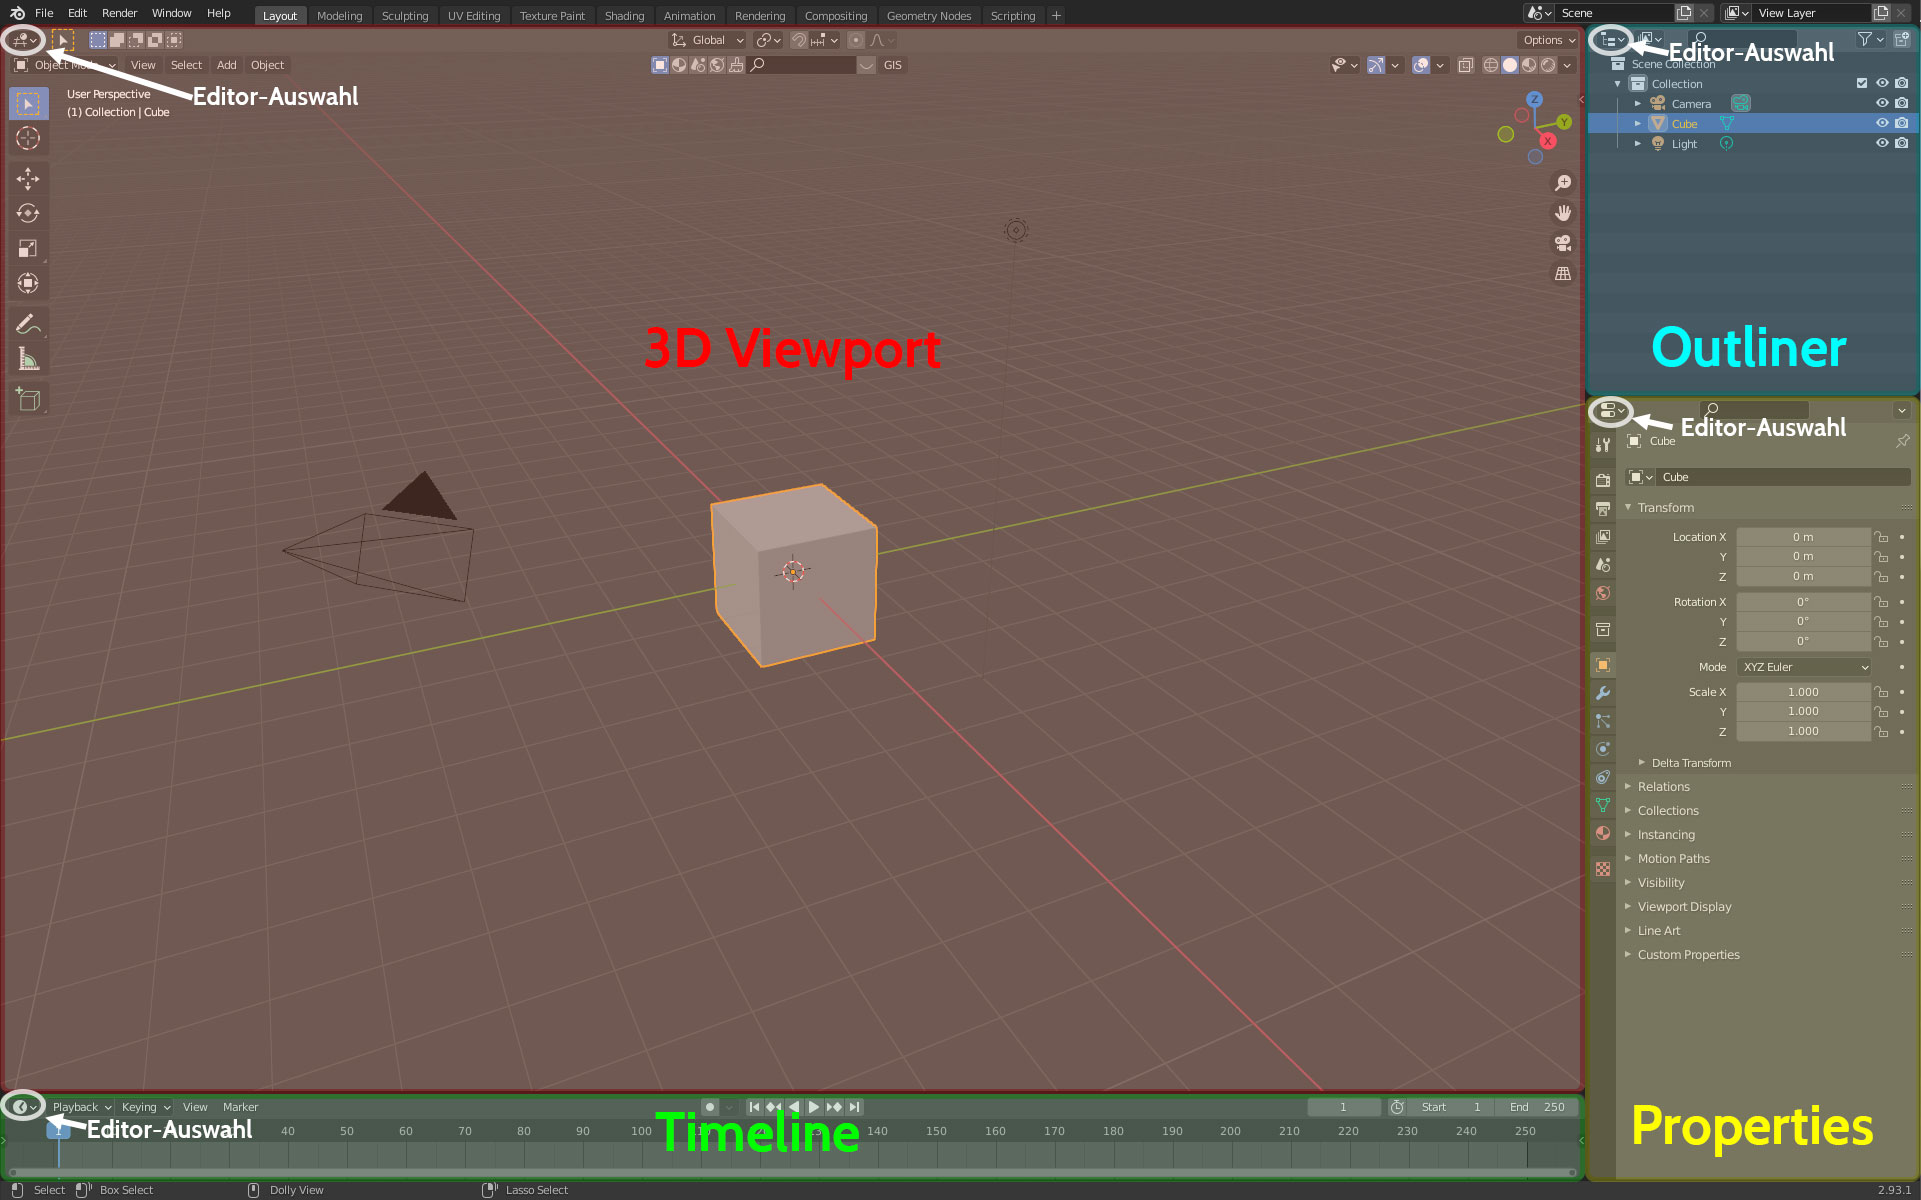
\includegraphics{Chapters/Images/Chapter_1/1_2_Default_Areal.jpg}

\caption{\label{fig-1_2}Default-Aufteilung der Arbeitsbereiche.}

\end{figure}%

\section{Übersicht über die Editor-Fenster von
Blender}\label{uxfcbersicht-uxfcber-die-editor-fenster-von-blender}

\marginnote{Editoren austauschen}

In jedem Editor-Areal befindet sich in der linken oberen Ecke eine
Schaltfläche. Durch das Drücken dieser Schaltfläche wird ein
Dropdown-Menü geöffnet. Darin sind alle verfügbaren Editoren
aufgelistet. Indem ein anderer Editor ausgetauscht wird, wechselt die
Anzeige in diesem Areal zu dem ausgewählten Editor.

\begin{figure}

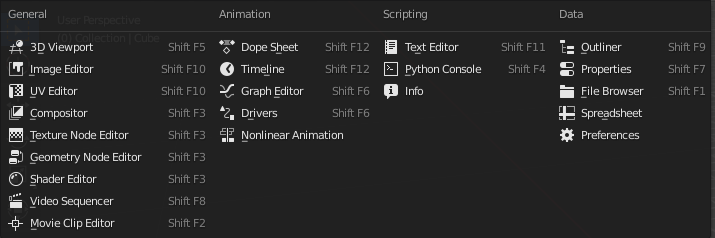
\includegraphics{Chapters/Images/Chapter_1/1_3_Editor_Select.png}

\caption{\label{fig-1_3}Die Auswahl an verschiedenen Editoren, welche
Blender standardmässig mit sich bringt.}

\end{figure}%

\subsection{3D Viewport}\label{d-viewport}

\marginnote{«General» Edito-ren}

Der 3D-Viewport stellt die bearbeiteten Szenen und die dazugehörigen
3D-Objekte dar. Er bietet die Möglichkeit zur direkten Interaktion mit
diesen Objekten und ist für das Modellieren von Objekten essenziell. Bei
der Arbeit mit 3D-Objekten ist es der wichtigste Editor.

\subsection{Image Editor}\label{image-editor}

Anhand des Image-Editors können 2D-Grafiken betrachtet und bearbeitet
werden. Gerenderte Bilder werden ebenfalls in diesem Editor angezeigt.

\subsection{UV Editor}\label{uv-editor}

Der UV-Editor wird verwendet, um den Flächen von Objekten eine bestimmte
Position auf einer Textur (sogenannte UVs) zuzuweisen oder dessen
Zuweisung zu betrachten.

\subsection{Compositor}\label{compositor}

Mithilfe des Compositors lassen sich Bilder, welche beim Rendern
erstellt werden, nachträglichen Bearbeitungen unterziehen. Auch externe
Bilder können hier bearbeitet werden. Die Bearbeitung erfolgt mittels
einer visuellen Programmiersprache.

\subsection{Texture Node Editor}\label{texture-node-editor}

Mithilfe des Texture-Node-Editors können Texturen anhand einer visuellen
Programmiersprache erstellt werden. Dieser Editor wird allerdings in
Zukunft durch andere Bearbeitungsoptionen ersetzt.

\subsection{Geometry Node Editor}\label{geometry-node-editor}

Der Geometry-Node-Editor ermöglicht das Bearbeiten von Objekten mittels
einer visuellen Programmiersprache. Innerhalb dieses Editors erfolgt
dabei die Programmierung der geometrischen Figuren, während die
Darstellung der Figuren im 3D-Viewport erfolgt. Bei den Geometry Nodes
handelt es sich um eine neue Funktion von Blender.

\subsection{Shader Editor}\label{shader-editor}

Mithilfe des Shader-Editors können die Materialien, welche einem
dreidimensionalen Objekt zugewiesen sind, bearbeitet werden. Dadurch
lässt sich bearbeiten, wie die Oberfläche eines Objektes aussieht. Die
Bearbeitung erfolgt hier mittels einer visuellen Programmiersprache.
Innerhalb dieses Editors werden lediglich die Einstellungen für die
Materialien gemacht. Um die Auswirkungen der Materialien zu sehen, wird
der 3D-Viewport verwendet.

\subsection{Video Sequencer}\label{video-sequencer}

Mithilfe des Video-Sequencers können Videoaufnahmen bearbeitet werden.
Dieser Editor verfügt zusätzlich über eine Vorschau-Option, mit der sich
die Videos direkt betrachten lassen.

\subsection{Movie Clip Editor}\label{movie-clip-editor}

Der Movie-Clip-Editor ermöglicht das Erfassen von Bewegungen in Filmen,
sodass diese Bewegungen beispielsweise auch auf 3D-Objekte angewendet
werden können. Zudem lassen sich hier auch Videos maskieren.

\subsection{Dope Sheet}\label{dope-sheet}

\marginnote{Editoren für Animationen}

Das Dope-Sheet stellt einzelne Animationspunkte eines Projektes in einem
zeitlichen Ablauf tabellarisch dar. Dies basiert auf der früher
angewendeten Planung von handgezeichneten Animationen.

\subsection{Timeline}\label{timeline}

Die Timeline stellt einen zeitlichen Verlauf von Animationen dar. Für
die ausgewählten Objekte wird hier durch Punkte dargestellt, wann eine
Animation im Zeitstrang starten oder enden soll. Zudem befindet sich
hier auch eine Schaltfläche, um Animationen abspielen zu lassen.

\subsection{Graph Editor}\label{graph-editor}

Mittels des Graph-Editors können Animationen über die Zeit hinweg
verfeinert werden. Hierfür werden die einzelnen Animationen mittels
Grafen dargestellt. Durch eine Veränderung dieser Grafen wird die
Animation verfeinert.

\subsection{Drivers}\label{drivers}

Der Driver-Editor ermöglicht es, Animationen gezielt zu steuern. Dabei
können die Eigenschaften eines Objektes verwendet werden, um ein anderes
Objekt zu steuern.

\subsection{Nonlinear Animation}\label{nonlinear-animation}

Mittels des Editors für nonlineare Animationen können Animationen
ausserhalb eines linearen Ablaufes gesteuert werden. Dies kommt etwa bei
komplexeren Veränderungen von Szenen zum Einsatz.

\subsection{Text Editor}\label{text-editor}

\marginnote{Editoren für Programmier-Skripte}

Im Text-Editor können Textdokumente eingesehen und erstellt werden.
Diese Textdokumente können auch verwendet werden, um mittels der
Programmiersprache Python Funktionen für Blender zu verfassen. Zudem
können im Text-Editor auch direkt Programmfunktionen in Textdokumenten
ausgeführt werden.

\subsection{Python Console}\label{python-console}

Anhand der Python-Konsole lassen sich Codes in der Programmiersprache
von Python eingeben. Blender führt diese Codes anschliessend aus.

\subsection{Info}\label{info}

Im Info-Editor werden durchgeführte Aktionen in der
Python-Programmiersprache nacheinander aufgelistet. Hier lassen sich
auch Fehlermeldungen und Warnungen nachträglich einsehen.

\subsection{Outliner}\label{outliner}

\marginnote{«Data»-Editoren}

Im Outliner werden alle Daten, welche sich in einer Blender-Datei
befinden, aufgelistet. Hier lassen sich Objekte innerhalb einer Szene
auswählen oder in Ordnerstrukturen (sogenannten Collections) anordnen
und gruppieren.

\subsection{Properties}\label{properties}

Im Properties Editor lassen sich eine Reihe von Einstellungen machen. Es
umfasst neben Einstellungen zu einem aktuell ausgewählten Objekt auch
Einstellungen zum Rendern, zur Szenengestaltung oder zu physikalischen
Simulationen.

\subsection{File Browser}\label{file-browser}

Mithilfe des File-Browsers lassen sich Dateien auf dem Computer
darstellen und suchen. Dadurch können Dokumente direkt in die Szene
hineingezogen werden, ohne dass Blender minimiert werden muss. Zudem
können hier auch Dateien abgespeichert werden.

\subsection{Spreadsheet}\label{spreadsheet}

Mithilfe des Spreadsheets lassen sich alle Datenpunkte eines Objektes
mitsamt deren Positionen in der 3D-Welt angeben. Nebst den Punkten
können auch die Positionen der verschiedenen Kanten und Flächen von
Objekten angezeigt werden.

\subsection{Preferences}\label{preferences}

Unter den Preferences lassen sich die Einstellungen von Blender
bearbeiten. Die Preferences können auch unter «\emph{Edit \textbar{}
Preferences}» geöffnet werden.

\section{Vorgefertigte
Editor-Anordnungen}\label{vorgefertigte-editor-anordnungen}

\marginnote{Schnelle Auswahl von Editoren mittels Editor-Anordnungen}

In der Menüleiste sind für verschiedene Arbeitsschritte bei der
3D-Modellierung bereits vorgefertigte Ansichtsoptionen verfügbar. Durch
einen Klick auf den Reiter «\emph{Texture Paint}» wird beispielsweise
eine Anordnung gezeigt, welche ideal dafür ist, um ein Objekt mit einer
Textur zu bemalen. In diesem Falle wird beispielsweise nebst dem
3D-Viewport auch der Image Editor geöffnet. Mittels der Registerkarte
«+» können zudem weitere Editor-Anordnungen basierend auf einer Vorlage
für die Schnellauswahl hinzugefügt werden.

\section{Neuanordnen der
Editor-Areale}\label{neuanordnen-der-editor-areale}

\marginnote{Grösse der Edito-ren verändern}

Die einzelnen Editor-Fenster können nicht nur beliebig ausgetauscht
werden, sondern auch nach eigenem Belieben vergrössert oder verkleinert
werden. In den Abgrenzungsbereichen zwischen den Fenstern verändert sich
der Mauszeiger. Von dort aus lassen sich die Editor-Areale durch Hin-
und Herziehen vergrössern oder verkleinern.

\marginnote{Neue Editoren öffnen}

In den Ecken der einzelnen Editor-Fenster gibt es zudem die Möglichkeit,
durch Ziehen der Ecke in eine Richtung das Fenster in zwei Editoren
aufzuteilen. Wenn dabei gleichzeitig die \kbd{Shift}-Taste gedrückt
wird, wird derselbe Editor in einem neuen, einzelnen Fenster geöffnet.

\marginnote{Editor-Areal schliessen}

Um ein Editor-Fenster zu schliessen, wird jeweils ein anderes
Editor-Fenster über das zu schliessende Fenster gezogen. Dadurch werden
die beiden Fenster verbunden. Um zwei Fenster zu verbinden, wird eine
der beiden Ecken, welche sich zwischen den beiden Fenstern befindet,
ausgewählt und das zu behaltende Fenster über das zu entfernende Fenster
gezogen. Dies ist manchmal etwas knifflig, da die Aktion ähnlich zum
Öffnen von neuen Fenstern ist.

Übung 1: Editor-Auswahl

\textbf{Übung 1.1}

Ordnen Sie die Arbeitsoberfläche entsprechend der nachfolgenden
Abbildung an.

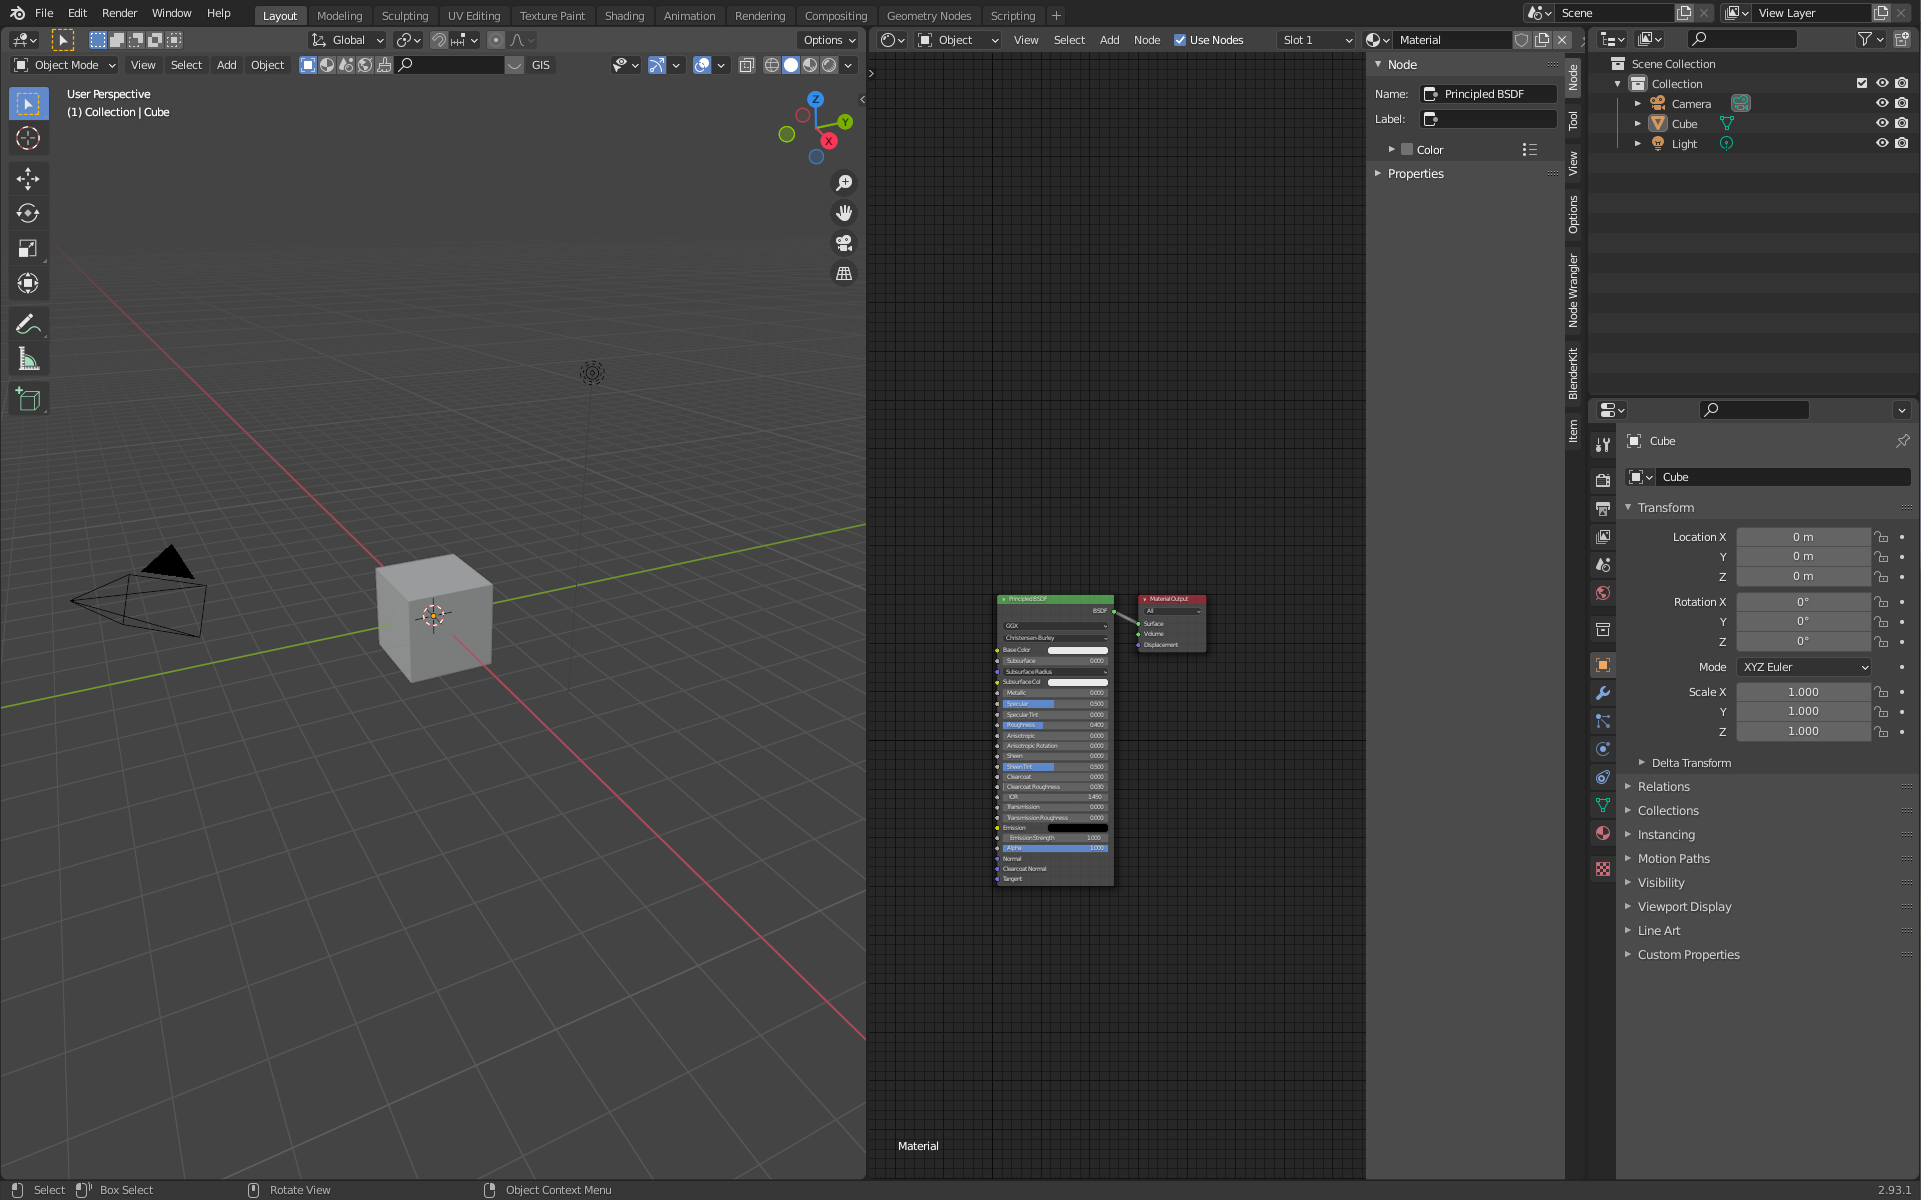
\includegraphics{Chapters/Images/Chapter_1/Exercise_1_1.png}\hfill

\textbf{Übung 1.2}

Ordnen Sie die Arbeitsoberfläche entsprechend der nachfolgenden
Abbildung an.

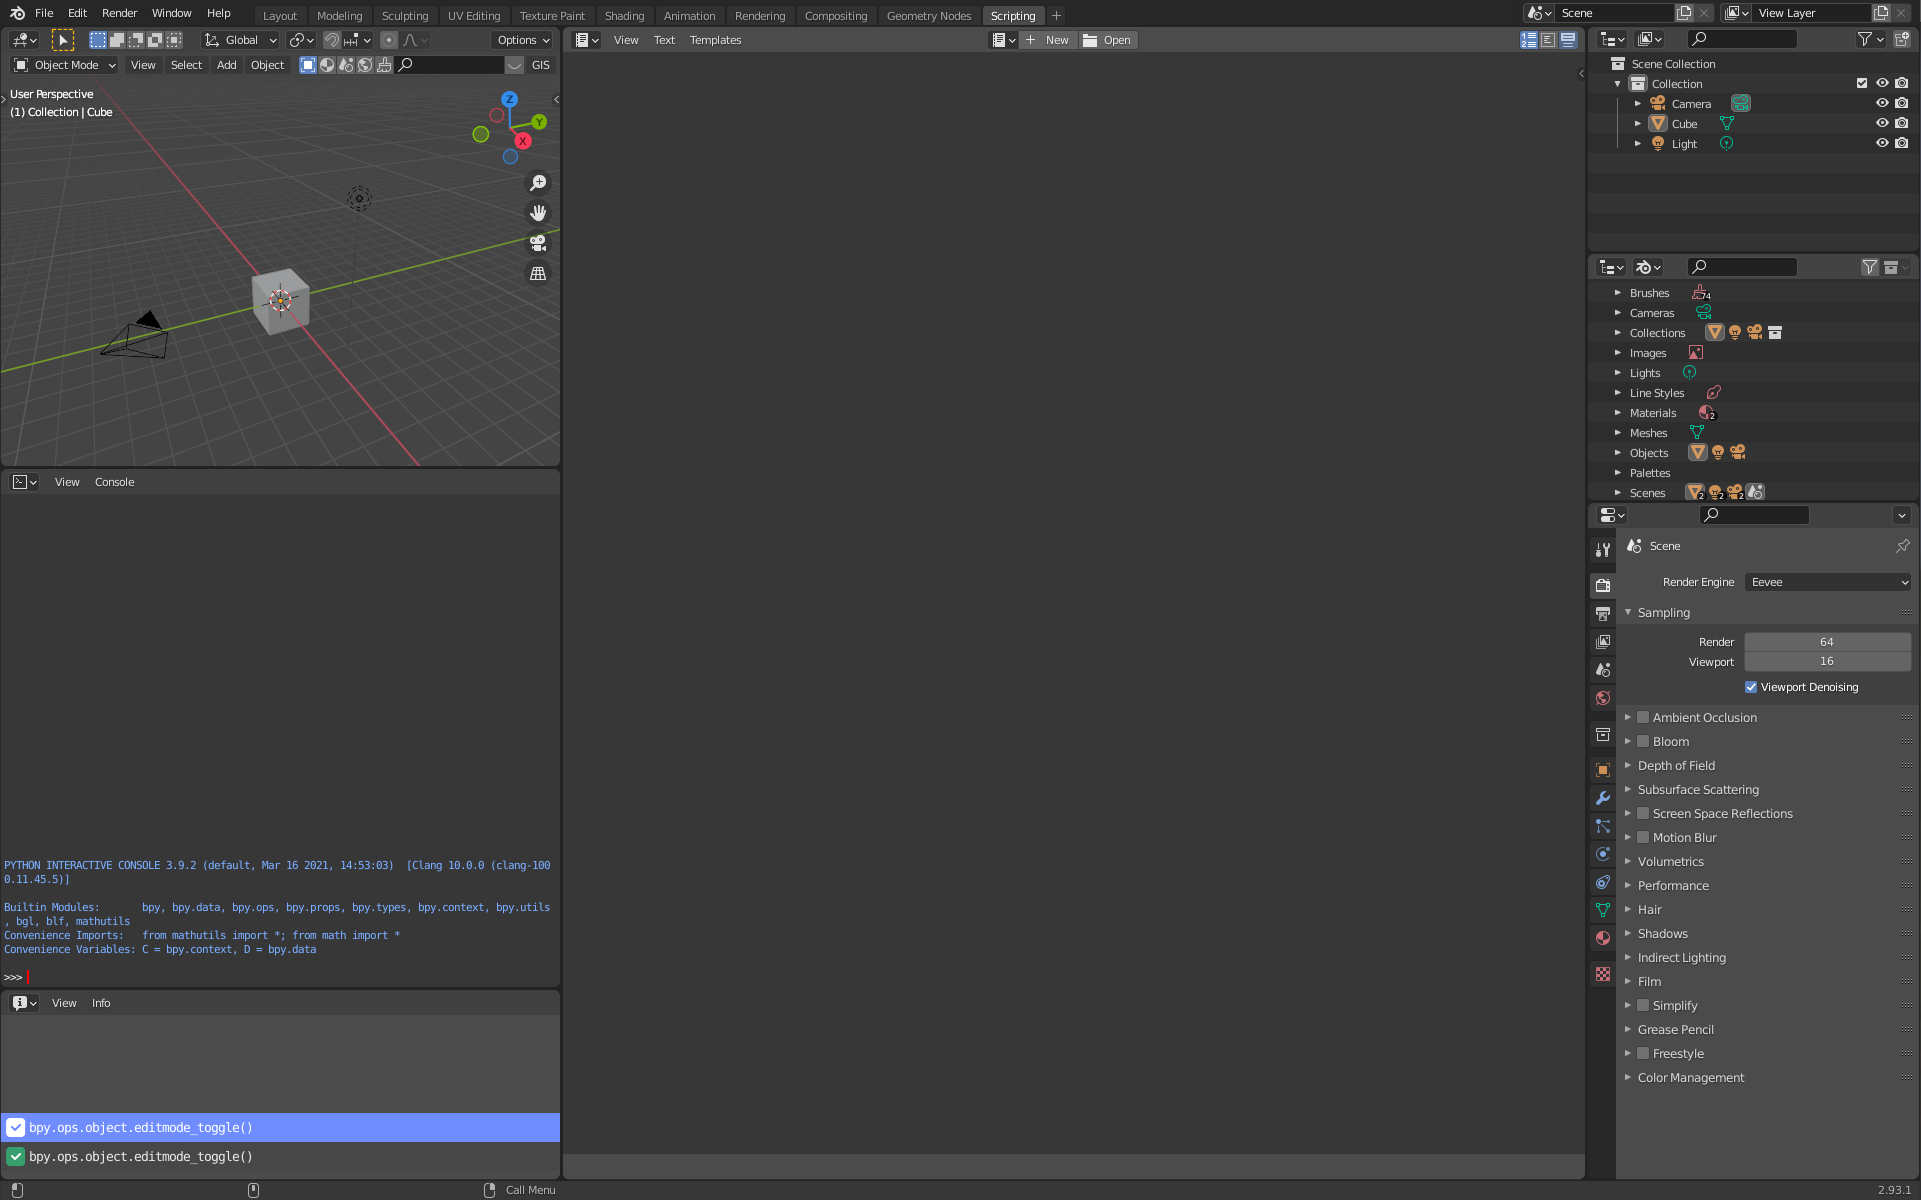
\includegraphics{Chapters/Images/Chapter_1/Exercise_1_2.png}\hfill

\chapter{2. Die Arbeitsoberfläche des
3D-Viewports}\label{die-arbeitsoberfluxe4che-des-3d-viewports}

\marginnote{Funktion des 3D-Viewports}

Der 3D-Viewport stellt eine der wichtigsten Arbeitsoberflächen in
Blender dar. In ihm werden die 3D-Objekte sowie die Szenen, in denen sie
integriert werden, angezeigt. Zudem werden im 3D-Viewport eine Reihe
anderer Einstellungen dargestellt, welche in anderen Editoren
konfiguriert werden können. Die Bearbeitung der grundlegenden Struktur
von 3D-Objekten erfolgt in der Regel direkt im 3D-Viewport. Der
Arbeitsbereich des 3D-Viewports lässt sich in verschiedene Areale
aufteilen, welche nachfolgend genauer betrachtet werden.

\section{Toolbar}\label{toolbar}

\marginnote{Toolbars}

Die Toolbar befindet sich auf der linken Seite der 3D-View. Allerdings
sind Toolbars auch in anderen Editoren anzutreffen. Die Toolbars lassen
sich jeweils mit der Taste \kbd{T} ein- und ausblenden. Da es auch im
3D-Viewport verschiedene Bearbeitungsmöglichkeiten gibt, variieren die
Elemente in der Toolbar abhängig vom Bearbeitungsmodus. Diese sind
entweder per Mausklick über diese Toolbar oder mithilfe von
Tastenkombinationen aufrufbar. In diesem Kurs wird vor allem auf
Tastenkombinationen verwiesen, wenn Operationen durchgeführt werden.

\section{Sidebar}\label{sidebar}

\marginnote{Sidebars}

Die Sidebar befindet sich auf der rechten Seite des Viewport-Displays,
muss allerdings noch mit der Taste \kbd{N} geöffnet werden. Mit dieser
Taste lässt sich die Sidebar ebenfalls wieder verbergen. Die Sidebar ist
auch in anderen Editoren anzutreffen und wird dort ebenfalls mit der
Taste\kbd{N} ein- und ausgeblendet. Die Sidebar ist zudem anhand von
Registerkarten in zusätzliche Kategorien eingeordnet. Unter dem Register
«\emph{Item}» können etwa Einstellungen zum aktuell ausgewählten Objekt
betrachtet und verändert werden, im Register «\emph{Tool}» können
Einstellungen zum aktuell ausgewählten Werkzeug verfeinert werden und
unter dem Register «\emph{View}» können Einstellungen zur Ansicht
betrachtet und verfeinert werden.

\section{Header}\label{header}

Im Header sind zusätzliche Einstellungen aufzufinden. Diese können nicht
nur zwischen den einzelnen Editoren variieren, sondern auch zwischen den
einzelnen Bearbeitungsmodi inner-halb der 3D-View.

\subsection{Aktions-Einstellungen}\label{aktions-einstellungen}

In der oberen linken Ecke, direkt neben dem Bedienfeld für die Auswahl
des Editors, befinden sich Einstellungsmöglichkeiten, welche basierend
auf der aktuell durchgeführten Aktion verfeinert werden können.

\begin{figure}


\includegraphics{Chapters/Images/Chapter_2/2_1_Actions_Parameters.png}

\caption{\label{fig-2_1}Aktions-Einstellungen am Beispiel der Auswahl.}

\end{figure}%

\subsection{Erweiterte Hilfsmittel zur
Bearbeitung}\label{erweiterte-hilfsmittel-zur-bearbeitung}

\marginnote{Hilfsmittel zur Bearbeitung von Objekten}

In der Mitte des Headers befinden sich eine Reihe von erweiterten
Einstellungen, welche bei der Objektbearbeitung als Hilfsmittel
verwendet werden können. Hierzu gehört beispielsweise die proportionale
Bearbeitung von Objekten oder das Festlegen von Bezugspunkten für
Transformationen. Diese Hilfsmittel werden in einem späteren Kapitel
ausführlich behandelt.

\begin{figure}

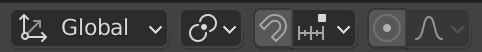
\includegraphics{Chapters/Images/Chapter_2/2_2_Extended_helper.png}

\caption{\label{fig-2_2}Erweiterte Hilfsmittel.}

\end{figure}%

\subsection{Bearbeitungsmodus}\label{bearbeitungsmodus}

\marginnote{Auswahl des Bearbeitungsmodus}

In der Zeile unterhalb des Headers befindet sich links das Menü zur
Auswahl des Bearbeitungsmodus. Dabei wird definiert, wie das aktuelle
Objekt bearbeitet werden soll. So kann beispielsweise im Object-Mode das
Objekt als Ganzes bearbeitet werden, während im Edit-Mode die Struktur
des Objektes bearbeitet werden kann.

\begin{figure}


\includegraphics{Chapters/Images/Chapter_2/2_3_Edit_Mode_Choice.png}

\caption{\label{fig-2_3}Auswahl des Bearbeitungsmodus.}

\end{figure}%

\subsection{Anzeige-Optionen}\label{anzeige-optionen}

\marginnote{Anzeige-Optionen}

In der rechten oberen Ecke befinden sich Optionen zur Darstellung der
Objekte in der 3D-View. Diese umfassen:

\begin{itemize}
\tightlist
\item
  View Object Types
\item
  Show Gizmo
\item
  Show Overlay
\item
  Toggle X-Ray
\item
  Viewport Shading
\end{itemize}

\subsubsection{View Object Types}\label{view-object-types}

\marginnote{Ein- und Ausblen-den von Objektarten}

Hier lassen sich verschiedene Arten von Objekten alle gemeinsam
innerhalb einer Szene verstecken, indem das Auge zu der entsprechenden
Objektart abgewählt wird. Durch das Abwählen des Auges neben dem
Objekttyp «\emph{Camera}» werde etwa alle Kameras aus der Szene
unsichtbar gemacht. Die Objekte sind allerdings noch vorhanden und
weisen immer noch dieselbe Funktion auf -- sie werden lediglich nicht
mehr im 3D-Viewport angezeigt. Neben dem Auge lässt sich zudem anhand
der Schaltfläche mit einem abgebildeten Cursor einstellen, dass die
entsprechenden Objektarten nicht mehr auswählbar sind.

\begin{figure}


\includegraphics{Chapters/Images/Chapter_2/2_4_Icon_Viewobjecttypes.png}

\caption{\label{fig-2_4}View Object Types.}

\end{figure}%

\subsubsection{Show Gizmo}\label{show-gizmo}

\marginnote{Navigations-Tools ein- und ausblen-den}

Innerhalb dieser Option lassen sich in der oberen rechten Ecke Tools zur
Navigation mittels der Kamera ein- und ausblenden. Zudem kann hier die
Darstellung eines Gizmos bei der aktuellen Auswahl aktiviert werden.
Dieses Gizmo kann verwendet werden, um Objekte mittels der Maus zu
rotieren, zu skalieren oder zu bewegen.

\begin{figure}

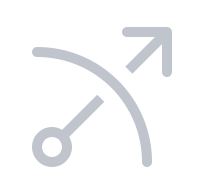
\includegraphics{Chapters/Images/Chapter_2/2_5_Icon_Show_Gizmos.png}

\caption{\label{fig-2_5}Show Gizmo.}

\end{figure}%

\subsubsection{Show Overlays}\label{show-overlays}

\marginnote{Orientierungsobjekte im Viewport ein- und ausblenden}

Durch die Deaktivierung der Viewport-Overlays wird im 3D-Viewport die
Ansicht bestimmter Hilfsmittel (beispielsweise die Achsen oder die
Markierung der aktuellen Auswahl) ausgeschal-tet. Im Dropdown-Menü lässt
sich zudem die Darstellung von einzelnen Hilfsmitteln individuell an-
und abwählen.

\begin{figure}


\includegraphics{Chapters/Images/Chapter_2/2_6_Icon_Showoverlays.png}

\caption{\label{fig-2_6}Show Overlays.}

\end{figure}%

\subsubsection{Toggle X-Ray}\label{toggle-x-ray}

\marginnote{Röntgenblick ein- und ausschalten}

Wenn die Schaltfläche «Toggle X-Ray» ausgewählt ist, erweitert sich die
Ansicht von Objekten, sodass durch sie hindurchgesehen werden kann. Dies
ermöglicht es etwa, dass auch ein Objekt, welches hinter einem anderen
Objekt verborgen liegt, betrachtet werden kann. Wenn diese Option
aktiviert ist, können zudem die verborgenen Objekte mittels eines
Mausklicks angewählt werden. Die Schaltfläche kann auch mit den Tasten
\kbd{Alt} + \kbd{Z} ein- und ausgeschaltet werden.

\begin{figure}


\includegraphics{Chapters/Images/Chapter_2/2_7_Icon_Xray.png}

\caption{\label{fig-2_7}Toggle X-Ray.}

\end{figure}%

\subsubsection{Viewport Shading}\label{viewport-shading}

\marginnote{Art der Objektdar-stellung im Viewport}

In der rechten oberen Ecke befinden sich vier Schaltflächen, um
einzustellen, welche Elemente bei der Darstellung der Objekte
berücksichtigt werden sollen. Je nach Auswahl werden dadurch die Objekte
unterschiedlich dargestellt:

\begin{itemize}
\tightlist
\item
  \textbf{Wireframe}: Die Objekte werden in ihrer Struktur als
  Gitternetz angezeigt, sodass deren Aufbaugitter klar ersichtlich wird.
  Hierbei werden die Flächen der Objekte nicht dargestellt.
\item
  \textbf{Solid}: Die Objekte werden als Ganzes dargestellt, sodass auch
  die Flächen sichtbar sind. Allerdings werden die verwendeten
  Materialien und Texturen nicht berücksichtigt.
\item
  \textbf{Material Preview}: Die Objekte werden als Ganzes dargestellt,
  inklusive deren Materialien und Texturen. Die Umgebung wird anhand von
  vorgefertigten Szenen und Umgebungen beleuchtet, sodass eine schnelle
  Vorschau möglich ist.
\item
  \textbf{Rendered}: Die Objekte werden als Ganzes dargestellt,
  inklusive deren Materialien und Texturen. Die Umgebung und die
  Beleuchtung entsprechen den Einstellungen der aktuellen Szene, sodass
  eine Vorschau für die gerenderte Szene möglich ist.
\end{itemize}

Alternativ kann die Taste \kbd{Z} gedrückt werden. Dadurch erscheint
beim Mauszeiger ein Menü mit allen vier Optionen zum Viewport Shading
zur Auswahl.

\begin{figure}


\includegraphics{Chapters/Images/Chapter_2/2_8_Icon_Shaderbuttons.png}

\caption{\label{fig-2_8}Schaltflächen für die Shading-Optionen im
Viewport.}

\end{figure}%

\section{Letzte Aktion verfeinern}\label{letzte-aktion-verfeinern}

\marginnote{Temporäres Menü zur Verfeinerung der letzten Aktion}

Wenn eine Aktion in Blender durchgeführt wird, erscheint in der linken
unteren Ecke des 3D-Viewports temporär ein Menü. Dieses Menü kann
aufgeklappt werden und bietet abhängig von der durchgeführten Aktion
eine Reihe Verfeinerungen. Zu beachten ist jedoch, dass dieses Menü
sofort wieder verschwindet, sobald ein Mausklick ausserhalb des Menüs
erfolgt. Um das Menü wieder erscheinen zu lassen, muss die Aktion
rückgängig gemacht und erneut durchgeführt werden.

\section{Dargestellte
Viewport-Overlays}\label{dargestellte-viewport-overlays}

\marginnote{Achsen}

Sofern die Ansicht der Viewport-Overlays aktiviert ist, werden im
3D-Viewport einige nützliche Dinge dargestellt. Zum einen werden die
verschiedenen drei Achsen in unterschiedlichen Farben vom Nullpunkt der
Szene aus dargestellt:

\begin{itemize}
\tightlist
\item
  X-Achse: rot
\item
  Y-Achse: grün
\item
  Z-Achse: blau
\end{itemize}

Zudem wird leicht schattiert ein Gitternetz dargestellt, bei dem jedes
Quadrat eine Einheit von einem Meter darstellt. Wird aus der Szene
hinausgezoomt, werden diese Quadrate zunehmend kleiner, dafür werden
anschliessend quadratische Felder mit der Einheit von 10 Metern
sichtbar.

\begin{figure}

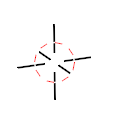
\includegraphics{Chapters/Images/Chapter_2/2_9_3DCursor.png}

\caption{\label{fig-2_9}3D-Cursor.}

\end{figure}%

\marginnote{3D-Cursor}

Innerhalb des 3D-Viewports ist ausserdem der 3D-Cursor sichtbar. Dieser
ist an einer bestimmten Position in der Szene platziert und dort mittels
eines rot-weissen Kreises dargestellt. Neu erstellte Objekte werden an
seiner Position in die Szene eingefügt und der 3D-Cursor kann als
Bezugspunkt für Transformationen verwendet werden.

\chapter{3. Navigation der Ansicht im
3D-Viewport}\label{navigation-der-ansicht-im-3d-viewport}

\marginnote{Navigation in der 3D-Ansicht}

Die Ansicht auf die Objekte im 3D-Viewport kann beliebig verändert
werden. Nebst der standardmässigen Ansichtssteuerung über die Maus kann
auch das Nummernfeld der Tastatur verwendet werden. In der Regel werden
beide Optionen verwendet. Die Navigation mit der Maus bietet tendenziell
eine grössere Flexibilität, während die Navigation mit der Tastatur eine
grössere Präzision ermöglicht.

\section{Navigation mit der Maus}\label{navigation-mit-der-maus}

\marginnote{Ansicht mit der Maus verändern}

Je nach Aufbau der verwendeten Computermaus unterscheidet sich die
Navigation durch den 3D-Viewport mit der Maus etwas. Bei einer
Computermaus mit einem Mausrad erfolgt die Navigation im 3D-Viewport
durch Mausbewegungen bei gedrückter Rad-Taste. Bei Trackpads oder Mäusen
mit integriertem Trackpad erfolgt die Navigation mittels
Wischbewegungen. Bei einer normalen Bewegung wird dabei lediglich die
Ansicht entsprechend der Bewegung rotiert. Durch gleichzeitiges Drücken
der \kbd{Shift}-Taste wird die Ansicht in die entsprechenden Richtungen
bewegt (ohne eine Rotation). Mittels gedrückter \kbd{Ctrl}-Taste kann
durch die Mausbewegung hinein- oder hinausgezoomt werden. Durch das
Drehen des Mausrads wird die Ansicht ebenfalls hinein- oder
hinausgezoomt.

\section{Navigation mit der Tastatur}\label{navigation-mit-der-tastatur}

\marginnote{Emulation des Nummernblocks}

Nebst der Maus kann auch die Tastatur verwendet werden, um die Ansicht
zu verändern. Diese Option ergibt sich allerdings nur, wenn man über
einen Nummernblock verfügt. Wenn kein Nummernblock zur Verfügung steht,
lassen sich auch die Zahlen-Tasten oberhalb der Buchstaben für die
Navigation verwenden. Hierfür muss allerdings in den
Benutzereinstellungen («\emph{Edit \textbar{} Preferences}») in den
Einstellungen zum «\emph{Input}» beim Keyboard-Reiter die Einstellung
«\emph{Emulate Numpad}» aktiviert werden.

\marginnote{Rotieren und Drehen der Ansicht}

Mittels der Tasten \kbd{2}, \kbd{4}, \kbd{6} und \kbd{8} kann die
Ansicht entsprechend ihrer relativen Anordnung auf dem Nummernblock
rotiert werden: Die Taste \kbd{2} rotiert nach unten, die Taste \kbd{4}
nach links, die Taste \kbd{6} nach rechts und die Taste \kbd{8} nach
oben. Werden dieselben Tasten bei gedrückter \kbd{Ctrl}-Taste gedrückt,
wird die Ansicht in die entsprechende Richtung bewegt, ohne eine
Rotation durchzuführen. Mittels gedrückter \kbd{Shift}-Taste kann die
Ansicht durch die Taste \kbd{6} zudem im Uhrzeigersinn und mittels der
Taste \kbd{4} gegen den Uhrzeigersinn gedreht werden. Um näher
hineinzuzoomen wird die Taste \kbd{+} und zum Hinauszoomen die Taste
\kbd{-} verwendet.

\marginnote{Präzise Ansichten ansteuern}

Mittels der Taste \kbd{1} kann die Ansicht direkt in die Vorderansicht
gedreht werden. Die Ansicht erfolgt anschliessend entlang der Y-Achse.
Die Rückansicht ist mit der Tastenkombination \kbd{Ctrl} + \kbd{1}
einstellbar. Mittels der Taste wird die Seitenansicht -- von der rechten
Seite aus zum Objekt hingewählt. Das Objekt wird in diesem Falle entlang
der X-Achse betrachtet. Mit der Tastenkombination \kbd{Ctrl} + \kbd{3}
ist die Seitenansicht von der linken Seite aus einstellbar. Um die Szene
aus der Vogelperspektive zu betrachten, kann die Taste \kbd{7} gedrückt
werden. Hierbei erfolgt die Ansicht der Z-Achse entlang. Mittels der
Tastenkombination \kbd{Ctrl} + \kbd{7} erfolgt die Ansicht von unten.

\marginnote{Perspektivische und orthogonale Darstelung}

Jede der Ansichten kann auf zwei Arten erfolgen: perspektivisch oder
orthogonal. Die perspektivische Ansicht berücksichtigt
Tiefeninformationen, sodass weiter entfernte Objekte kleiner dargestellt
werden. Die orthogonale Perspektive ignoriert die Tiefeninformationen,
wodurch weiter entfernte Objekte gleich gross angezeigt werden wie
nähere gleich grosse Objekte auf der entsprechenden Achse. Diese
Perspektive hat den Vorteil, dass Objekte in ihrer geometrischen Form in
2D betrachtet werden können. Mittels der Taste \kbd{5} kann zwischen
diesen beiden Ansichtsmodi gewechselt werden.

\marginnote{Kamera-Ansicht}

Mittels der Taste \kbd{0} kann die Ansicht direkt in die Position der
Kamera gelegt werden. Dadurch wird die Szene genau so betrachtet, wie
sie im finalen Render betrachtet werden wird. Wenn in einer Szene keine
Kamera vorhanden ist, steht diese Ansicht nicht zur Verfügung.Wenn
mehrere Kameras vorhanden sind, wird jeweils die Kamera, welche die
aktive Render Kamera darstellt, anvisiert. Um die Kameraperspektive zu
verlassen kann die Ansicht mittels der Maus bewegt werden, oder erneut
die Taste \kbd{0} gedrückt werden.

Merke\ldots{}

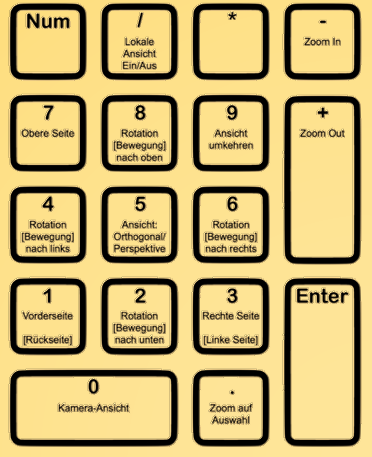
\includegraphics{Chapters/Images/Chapter_3/3_1_Number_Tabel.png}\hfill

\marginnote{Fokus auf ein Objekt}

In komplexeren Szenen kann es sein, dass man die Übersicht über die
Objekte verliert, oder dass sie sich gegenseitig im Weg stehen bei der
Ansicht. Mittels der Taste \kbd{.} auf dem Nummernblock wird die Ansicht
direkt auf ein ausgewähltes Objekt gezoomt. Diese Aktion lässt sich
nicht mit der Taste \kbd{.} ausserhalb des Nummernblocks emulieren.
Mittels der Taste \kbd{/} kann zudem die lokale Ansicht aktiviert
werden. In dieser Ansicht wird lediglich das ausgewählte Objekt
dargestellt, sodass es in komplexen Szenen besser betrachtet werden
kann. Allerdings muss anschliessend die Taste erneut gedrückt werden, um
die lokale Ansicht wieder zu verlassen. Auch diese Aktion lässt sich
nicht mit einer anderen Taste ausserhalb des Nummernblocks emulieren.

\section{Navigation mittels Gizmos}\label{navigation-mittels-gizmos}

Auf der rechten Seite des 3D-Viewports lassen sich zudem Schaltflächen
anzeigen, mit denen die Ansicht gesteuert werden kann. Um diese anzeigen
zu lassen, müssen die Gizmos eingeschaltet sein. Wird die linke
Maustaste auf das Kamera-Icon angewendet, wird die Kamera-Ansicht
aktiviert. Das Icon darunter, welches ein Gitternetz darstellt, dient
dem Wechsel zwischen perspektivischer und orthogonaler Ansicht. Die
beiden oberen Icons dienen dem Zoomen (mittels der Lupe) und dem Bewegen
der Ansicht (Hand). Hierfür muss das Icon angeklickt und die Maus
anschliessend bei weiterhin gedrückter Maustaste bewegt werden. Zuoberst
findet sich zudem ein Koordinatensystem, mit dem die Perspektive per
Mausklick oder mittels gedrückter Maustaste verändert werden kann.


\backmatter


\end{document}
